\chapter{General Overview}\label{chap:general_framework}
Our framework consists of several parts, each one dedicated to a different subtask and communicating with the others in order to achieve the final mission of landing on a moving platform. Figure \ref{fig:pipeline_diagram} shows the principal components of our framework. In this chapter we provide a brief introduction on each part, and in the following chapters we  discuss in details the parts developed in this thesis.
\begin{figure}[!ht]
    \centering
    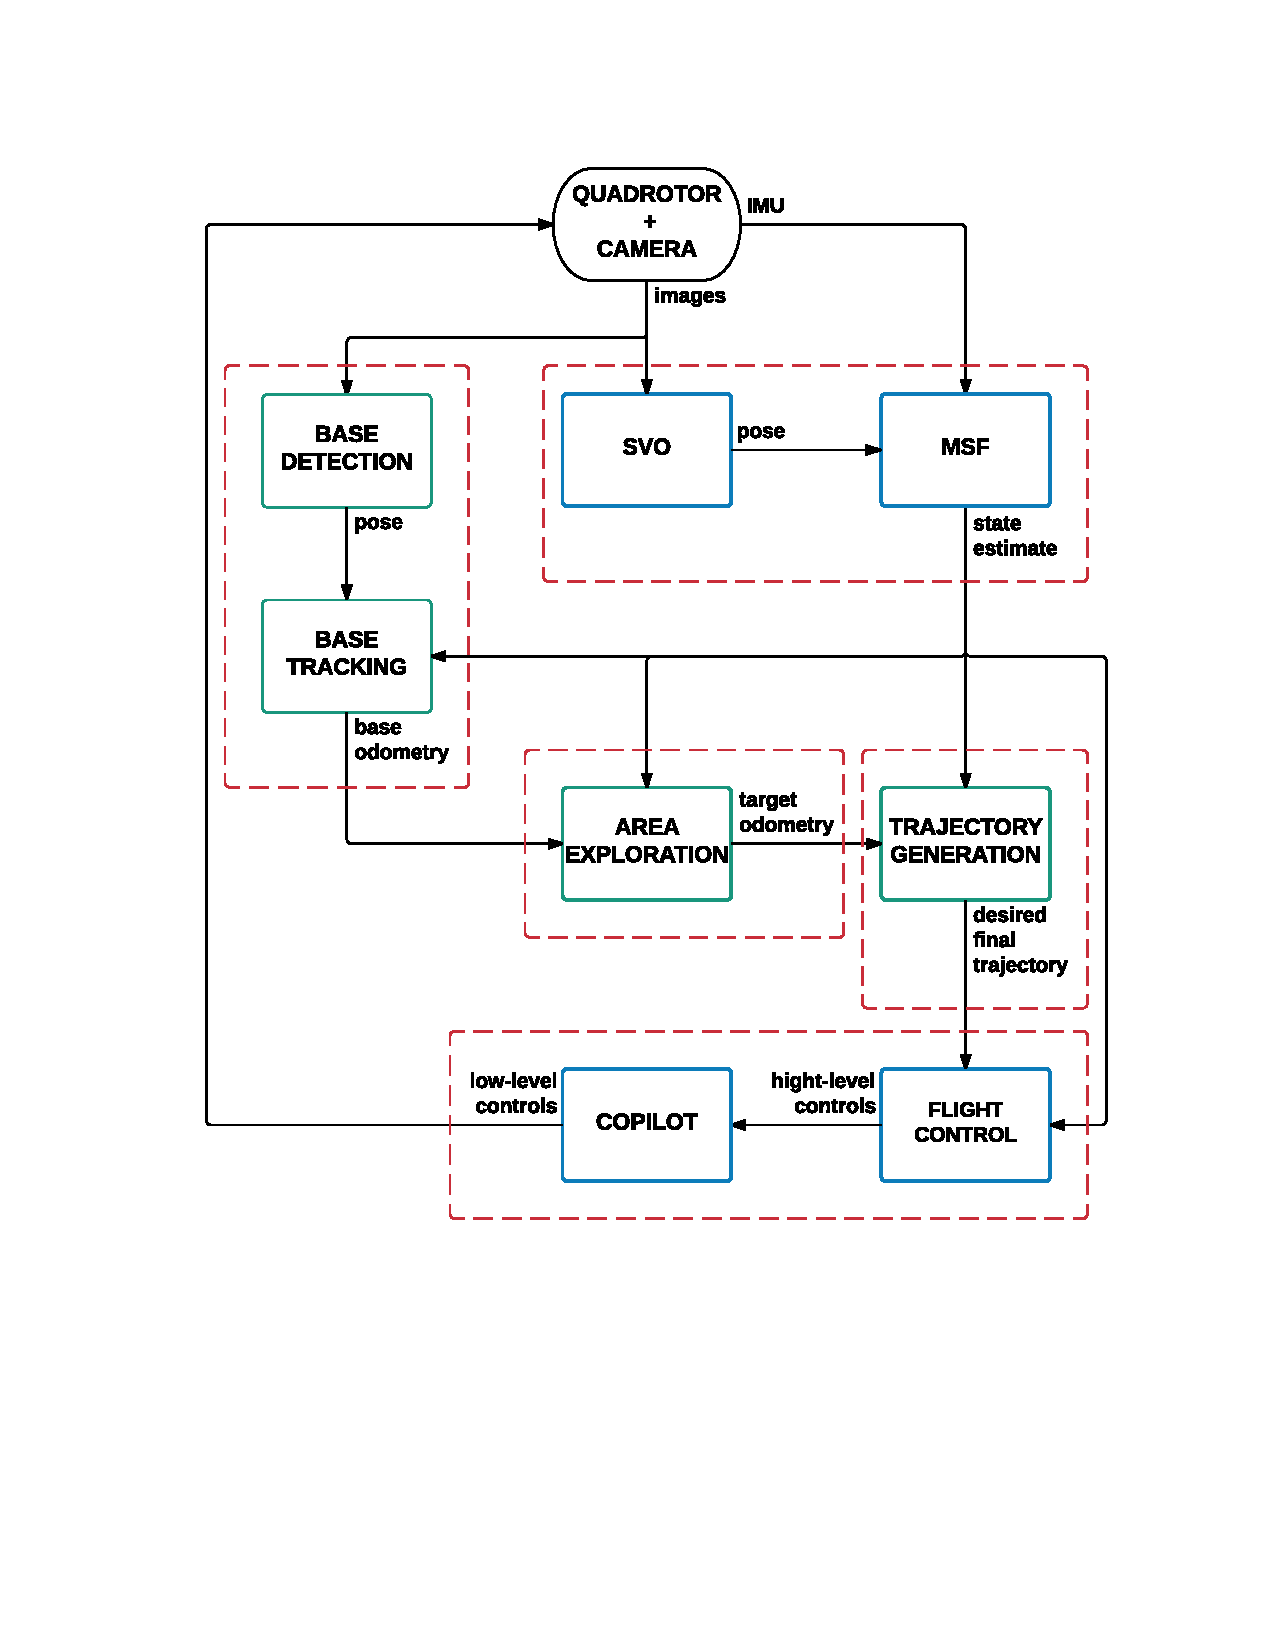
\includegraphics[width=1.0\textwidth]{img/pipeline_diagram.pdf}
    \caption{Pipeline of the framework. In blue the modules already implemented. In green the modules developed in this work.}
    \label{fig:pipeline_diagram}
\end{figure}

Our modular system, utilizes the Robot Operating System (ROS) \cite{ros} for interprocess communication. The platforms used in this project are capable of autonomous, vision-based flight utilizing only their on-board hardware resources and they do not need to rely on external communication infrastructure to accomplish their tasks. This is of critical importance in a field robotics scenario with uncertain communication reliability like the MBZIRC, , and our approach enables our platforms to perform their missions
autonomously without any dependence on external communication.

\section{SVO \& MSF} \label{sec:state_estimation}
The backbone of our system is an accurate state estimation pipeline provided by the visual odometry algorithm: Semidirect Monocular Visual Odometry (SVO) \cite{forster2014svo}. It provides a precise and robust pose estimate (3D position and orientation), and it runs at up to 55 frames per second on the onboard embedded computer of our flying robots. This vision-based pose estimate is fused with inertial data from an Intertial Measurement Unit (IMU) using the Multi-Sensor Fusion framework (MSF) \cite{lynen2013robust}.\\
The fusion of visual and inertial information provides a full state estimate of the UAVs.\\


\subsection{SVO}

SVO implements a semi-direct monocular visual odometry algorithm that estimates the motion of a camera in real time using sequential images. It combines the advantages of features extraction methods and direct approaches.\\
The standard techniques consist of extracting a sparse set of features in each image, matching them in successive frames using invariant feature descriptors, reconstructing camera motion and structure using epipolar geometry and finally, refining the pose and structure through reprojection error minimization. \\
On the other hand, appearance-based, or direct, methods estimate structure and motion directly from intensity values of the image: the camera pose relative to the previous frame is found through minimizing the photometric error between pixels.\\

%The majority of VO algorithms [12] follows this procedure, independent of the applied optimization framework. A reason for the success of these methods is the availability of robust feature detectors and descriptors that allow matching between images even at large inter-frame movement. The disadvantage of feature-based approaches is the reliance on detection and matching thresholds, the neccessity for robust estimation techniques to deal with wrong correspondences, and the fact that most feature detectors are optimized for speed rather than precision, such that drift in the motion estimate must be compensated by averaging over many feature-measurements.

%Direct methods that exploit all the information in the image, even from areas where gradients are small, have been shown to outperform feature-based methods in terms of robustness in scenes with little texture [14] or in the case of camera- defocus and motion blur [15]. The computation of the photometric error is more intensive than the reprojection error, as it involves warping and integrating large image regions. However, since direct methods operate directly on the intensitiy values of the image, the time for feature detection and invariant descriptor computation can be saved.


The semi-direct approach computes an initial guess of the relative camera motion and the feature correspondences using direct methods and concludes with a feature-based nonlinear reprojection-error refinement. This technique increases the computational speed due to the lack of feature-extraction at every frame (this operation is only required when a key-frame is selected to initialize new 3D points). Furthermore, it increases robustness and precision using many small patches instead of few large planar patches.
A new 3D point is added to the set used for motion estimation when its depth uncertainty becomes small enough. To estimate it, a probabilistic depth-filter is initialized for each 2D feature for which the corresponding 3D point is to be estimated. The filters are initialized with a large uncertainty in depth and at every subsequent frame it is updated in a Bayesian fashion.

%The proposed sparse model-based image alignment algorithm for motion estimation is related to model-based dense image alignmen.. However, we demonstrate that sparse information of depth is sufficient to get a rough estimate of the motion and to find feature- correspondences. As soon as feature correspondences and an initial estimate of the camera pose are established, the algorithm continues using only point-features; hence, the name “semi-direct”. This switch allows us to rely on fast and established frameworks for bundle adjustment.
%A Bayesian filter that explicitly models outlier measurements is used to estimate the depth at feature locations. A 3D point is only inserted in the map when the corresponding depth-filter has converged, which requires multiple measurements. The result is a map with few outliers and points that can be tracked reliably.

%eliminates the need of costly feature extraction and robust matching techniques for motion estimation. The algorithm operates directly on pixel intensities, which results in subpixel precision at high frame-rates.

%A probabilistic mapping method that explicitly models outlier measurements is used to estimate 3D points, which results in fewer outliers and more reliable points.

%Precise and high frame-rate motion estimation brings increased robustness in scenes of little, repetitive, and high-frequency texture.

\subsection{MSF}
MSF implements an Iterated Extended Kalman Filter (IEKF) \cite{bell1993iterated} over variable sized windows of updates. In the IEKF  the state prediction is driven by IMU data, while the update step can be of any nature. In our case we use the pose estimation given by SVO.\\
MSF has a modular structure that can support and merge an arbitrary number of sensors providing relative or absolute measurements (pose, position, pressure, etc). Furthermore, it estimates the extrinsic calibration between sensors and tracks the cross covariance terms for relative updates. It also has an outlier rejection module for the update measures.\\
MSF can compensate for unknown and changing delays implementing further propagation: the state is predicted with IMU data and whenever it receives an update step (usually in the past because of delays) it collocates this measurement in a ring-buffer that considers the moment this data was taken. Then it propagates this measure in time in order to update the current estimation and covariance based on the past data. With this function the framework can give state estimation at IMU rate and without delay.


\section{Control}
To control the flight of the quadrotor we need an algorithm that given the current state of the UAV and a final desired state it calculate the input that bring and stabilize the quad on the desired final condition.\\
The controller of the quadrotor is split into a high-level part and a low-level part: the former enables the tracking of a desired  pose and velocity and gives the input to the letter that tracks a desired thrust and body rates.\\

\subsection{High level control}\label{sec:high_control}

The high level control takes as input: 
\begin{itemize}
\item $([\hat{x},\hat{y},\hat{z}],[\hat{\phi},\hat{\theta},\hat{\psi}],[\hat{v_x},\hat{v_y},\hat{v_z}],[\hat{p},\hat{q},\hat{r}])$: the current state estimate (position, orientation, velocity, angular velocity, respectively) , computed in the previous module;
\item $([x_\mathrm{ref},y_\mathrm{ref},z_\mathrm{ref}],[v_{x,\mathrm{ref}},v_{y,\mathrm{ref}},v_{z,\mathrm{ref}}],[a_{x,\mathrm{ref}},a_{y,\mathrm{ref}},a_{z,\mathrm{ref}}],[\psi_{\mathrm{ref}}])$: a reference state (position, velocity, acceleration, yaw) , that can be sampled from a trajectory that the UAV should track to perform a task.
\end{itemize}
The outputs of this module are:
\begin{itemize}
\item $c_\mathrm{des}$: the desired mass-normalized thrust;
%\item $(\phi_{des},\theta_{des},\psi_{des})$: the desired attitude or
\item $(p_\mathrm{des},q_\mathrm{des},r_\mathrm{des})$: the desired body rates;
\end{itemize}
which are sent to the low-level controller.\\

The high level controller is composed by a position controller followed by an attitude controller, running at 50Hz.

\subsubsection{Position controller}
PD controller with feedback terms on the reference position and velocity and feedfoward on the reference acceleration:
\begin{align}
\begin{bmatrix}
a_{x,\mathrm{des}}  \\[10pt]
a_{y,\mathrm{des}}  \\[10pt]
a_{z,\mathrm{des}}
\end{bmatrix} = \boldsymbol{P}_{pos}
\begin{bmatrix}
x_{\mathrm{ref}} - \hat{x} \\[10pt]
y_{\mathrm{ref}} - \hat{y}  \\[10pt]
z_{\mathrm{ref}} - \hat{z}
\end{bmatrix} + 
\boldsymbol{D}_{pos}
\begin{bmatrix}
v_{x,\mathrm{ref}} - \hat{v_x} \\[10pt]
v_{y,\mathrm{ref}} - \hat{v_y}  \\[10pt]
v_{z,\mathrm{ref}} - \hat{v_z}
\end{bmatrix}
+
\begin{bmatrix}
a_{x,\mathrm{ref}}  \\[10pt]
a_{y,\mathrm{ref}}  \\[10pt]
a_{z,\mathrm{ref}} - g
\end{bmatrix} ,
\label{eq:PDcontroller1}
\end{align}

where $\boldsymbol{P}_{pos} = diag(p_{xy} ,p_{xy} ,p_{z} )$ and $\boldsymbol{D}_{pos} = diag(d_{xy} ,d_{xy} ,d_{z} )$ are positive-definite gain matrices.

%\begin{align}
%\begin{bmatrix}
%ax_{des}  \\[10pt]
%ay_{des}  \\[10pt]
%az_{des}
%\end{bmatrix}
%= 
%\begin{bmatrix}
%p_{xy} (x_{ref} - \hat{x}) + d_{xy}(vx_{ref} - \hat{vx}) + ax_{ref}  \\[10pt]
%p_{xy} (y_{ref} - \hat{y}) + d_{xy}(vy-{ref} - \hat{vy}) + ay_{ref}  \\[10pt]
%p_{z} (z_{ref} - \hat{z}) + d_{z}(vz_{ref} - \hat{vz}) + az_{ref} - g 
%\end{bmatrix}
%\label{eq:PDcontroller2}
%\end{align}
Now is very simple to derive the desired normalized thrust  $c_{\mathrm{des}}$: it is the projection of  $\boldsymbol{a}_{\mathrm{des}}$  on the current $z$ axis of the UAV:
\begin{align}
c_{des} = \boldsymbol{a}_{\mathrm{des}} \cdot \boldsymbol{e}_z^B
\label{eq:thrust}
\end{align}

\subsubsection{Attitude controller}
The output of this controller is $a_{des}$ and together with $\psi_{ref}$ determine two degrees of freedom of the body orientation $(\phi_\mathrm{des},\theta_\mathrm{des},\psi_\mathrm{des})$: since the quadrotor can only accelerate along the z direction of the body, we want to align this axis  with the desired acceleration $ \boldsymbol{a}_{\mathrm{des}}$, so it enforce both $\phi_{\mathrm{des}}$ and $\theta_{\mathrm{des}}$. The third degree of freedom is given by $\psi_{\mathrm{ref}}$.\\
With some geometric calculations it easy to define $(p_{\mathrm{des}},q_{\mathrm{des}},r_{\mathrm{des}})$: these values are function of the current orientation $(\hat{\phi},\hat{\theta},\hat{\psi})$, the desired final orientation of the z axis $\boldsymbol{e}_{z,des}^B = \frac{  \boldsymbol{a}_{\mathrm{des}}}{||  \boldsymbol{a}_{\mathrm{des}}||}$ and the desired final yaw $\psi_{\mathrm{des}} = \psi_{\mathrm{res}}$. \\
We refer to \cite{faessler2015automatic} for further details.



%To calculate $p_{des}$ and $q_{des}$ the following calculations are computed:
%\begin{align}
%\begin{split}
%e_{z,des}^B = \frac{ a_{des}}{|| a_{des}||} \\[10pt]
%\alpha = \cos^{-1}{e_{z}^B \cdot e_{z,des}^B} \\[10pt]
%\boldsymbol{n} = \frac{e_{z}^B times e_{z,des}^B}{||e_{z}^B times e_{z,des}^B||}
%\end{split}
%\label{eq:thrust}
%\end{align}
%where $e_{z,des}^B$ is the desired orientation of the z axis, $\alpha$ is the error angle and $\boldsymbol{n} $ is the rotation axis

\subsection{Low level control}
The low level controller takes as input:
 \begin{itemize}
\item $c_{\mathrm{des}}$: the desired normalize thrust 
\item $(p_\mathrm{des},q_\mathrm{des},r_\mathrm{des})$: the desired body rates
\item $(\hat{p},\hat{q},\hat{r})$: the current estimate angular velocity
\end{itemize}
and gives in output:
\begin{itemize}
\item $(f_{1,des},f_{2,des},f_{3,des},f_{4,des})$: the desired rotor thrusts.
\end{itemize}

We can compute the desired torques $\boldsymbol{\tau}_{\mathrm{des}}$ with the feedback linerized scheme:
\begin{align}
\begin{bmatrix}
\tau_{p,\mathrm{des}}  \\[10pt]
\tau_{q,\mathrm{des}}  \\[10pt]
\tau_{r,\mathrm{des}}
\end{bmatrix} 
= \boldsymbol{J}\boldsymbol{P}_{att}
\begin{bmatrix}
p_{\mathrm{des}} - \hat{q} \\[10pt]
q_{\mathrm{des}} - \hat{q}  \\[10pt]
r_{\mathrm{des}} - \hat{r}
\end{bmatrix} + 
\begin{bmatrix}
\hat{q} \\[10pt]
\hat{q}  \\[10pt]
\hat{r}
\end{bmatrix}
\times
\boldsymbol{J}
\begin{bmatrix}
\hat{q} \\[10pt]
\hat{q} \\[10pt]
\hat{r}
\end{bmatrix} ,
\label{eq:torques}
\end{align}
where $\boldsymbol{P}_{att} = diag(p_{qp} ,p_{qp} ,p_{r} )$ is a definite-positive gain matrix and  $\boldsymbol{J} = diag(J_{xx} ,J_{yy} ,J_{zz} )$ is the inertia matrix for rotation around the center of mass.\\
Now to find the thrusts for each rotor we have to solve:
\begin{align}
\begin{bmatrix}
f_{1,des}  \\[10pt]
f_{2,des}  \\[10pt]
f_{3,des}  \\[10pt]
f_{4,des}  
\end{bmatrix} 
=
\begin{bmatrix}
\frac{1}{4\lambda_1} \big(m c_{\mathrm{des}} + \frac{\tau_{r,\mathrm{des}}}{\kappa} - \frac{\sqrt{2}\tau_{q,\mathrm{des}}}{l} + \frac{\sqrt{2}\tau_{p,\mathrm{des}}}{l}\big) \\[10pt]
\frac{1}{4\lambda_2} \big(m c_{\mathrm{des}} - \frac{\tau_{r,\mathrm{des}}}{\kappa} - \frac{\sqrt{2}\tau_{q,\mathrm{des}}}{l} - \frac{\sqrt{2}\tau_{p,\mathrm{des}}}{l}\big) \\[10pt]
\frac{1}{4\lambda_3} \big(m c_{\mathrm{des}} + \frac{\tau_{r,\mathrm{des}}}{\kappa} + \frac{\sqrt{2}\tau_{q,\mathrm{des}}}{l} - \frac{\sqrt{2}\tau_{p,\mathrm{des}}}{l}\big)\\[10pt]
\frac{1}{4\lambda_4} \big(m c_{\mathrm{des}} - \frac{\tau_{r,\mathrm{des}}}{\kappa} + \frac{\sqrt{2}\tau_{q,\mathrm{des}}}{l} + \frac{\sqrt{2}\tau_{p,\mathrm{des}}}{l}\big)
\end{bmatrix} ,
\label{eq:thrusts}
\end{align}
where $\kappa$ is the rotor-torque coefficient and $\lambda_i$ are the rotor fitness coefficients, $l$ is the arm length between the center of mass and the point in which the thrust is applied. \\
Depending on the chosen orientation of the body frame we have a different mapping between torques $\tau_{i,des}$ and thrusts $f_j$. Figure \ref{fig:bodyframe} shows how our coordinate system is oriented with respect to the 4 propellers.

\begin{figure}[!ht]
    \centering
    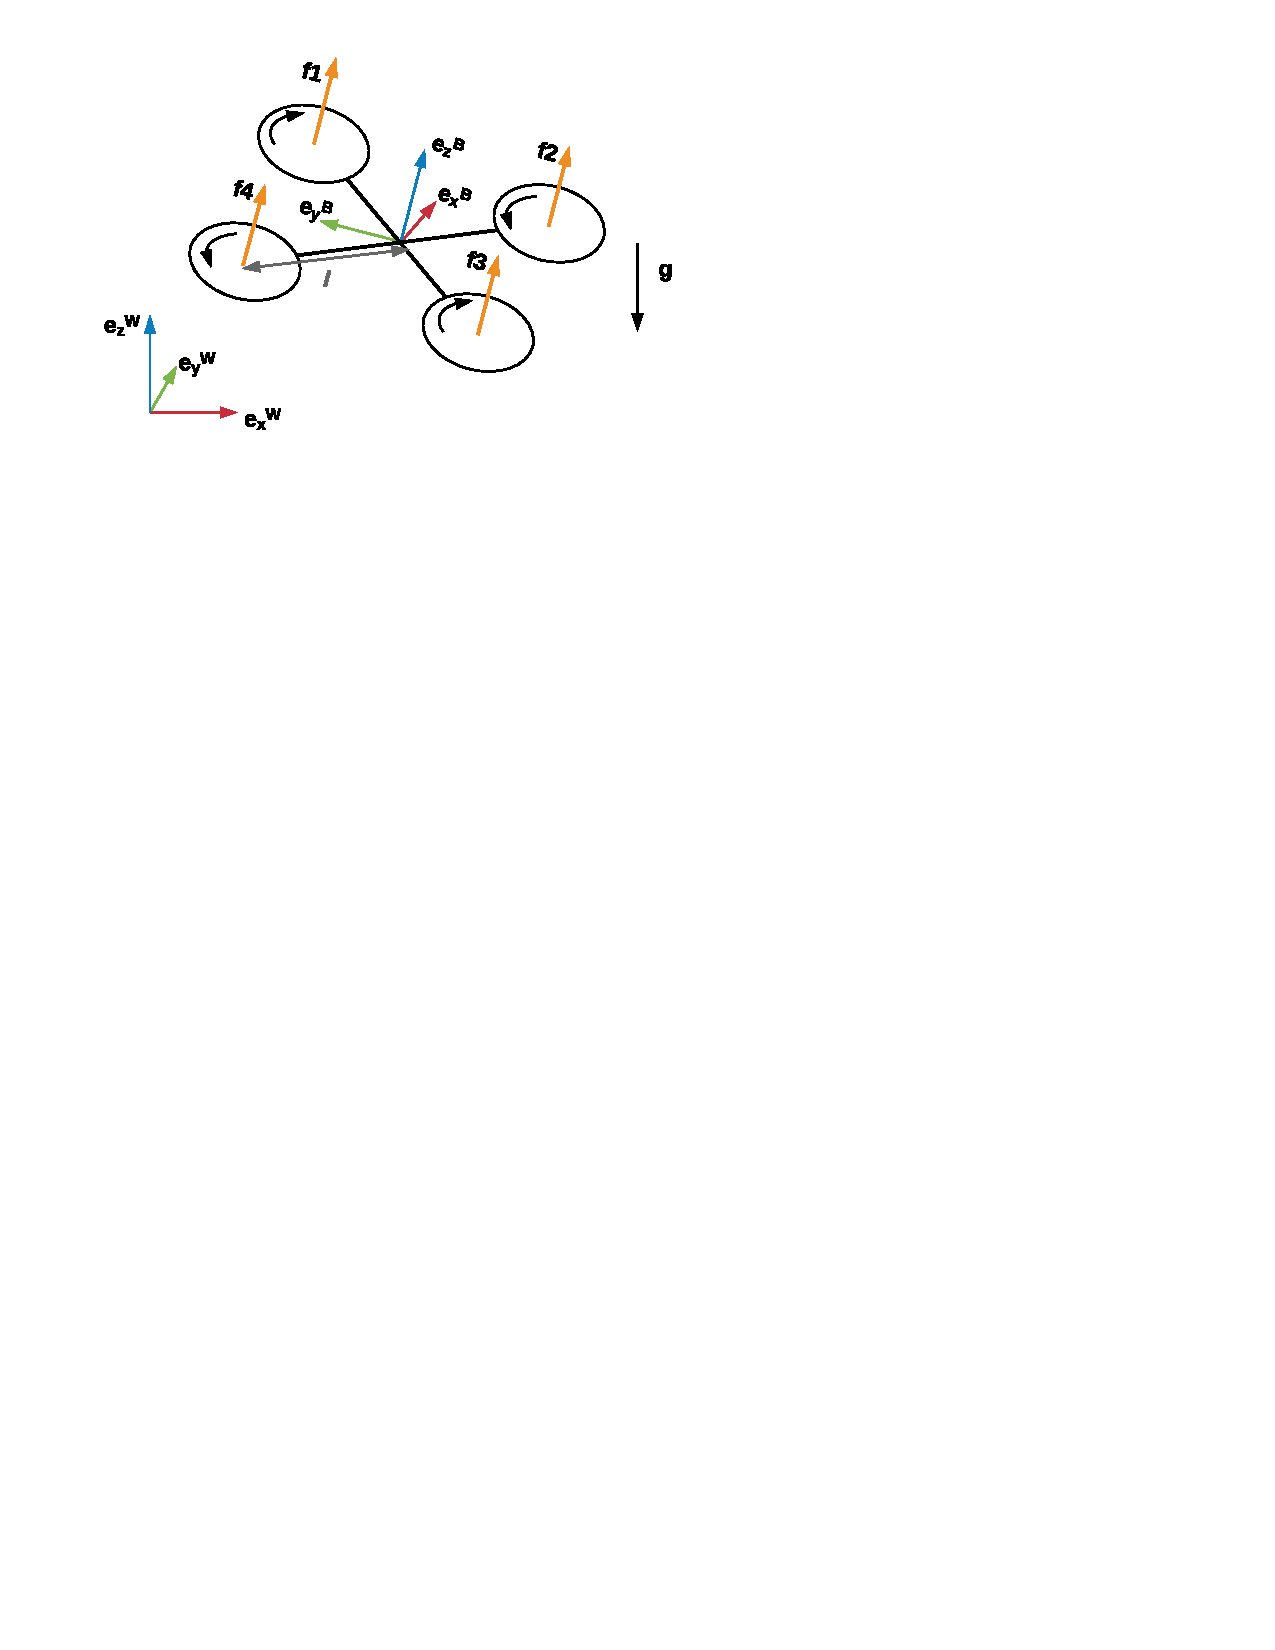
\includegraphics[width=0.7\textwidth]{img/quadrotor.pdf}
    \caption{Quadrotor with body coordinate frame and thrust forces.}
    \label{fig:bodyframe}
\end{figure}

\section{Base detection and tracking}\label{sec:base_estimation}
In order to land on the the moving platform, it is necessary to know where the base is at a specific time $t$. To do so we use images from the onboard camera to localize where the platform is with respect to the quadrotor. Then, given the position of the UAV with respect to the world frame, we can reconstruct the pose of the moving base in the global coordinate frame. \\
Now if a mathematical model of how the platform should move in the world frame  is available, we can combine the noisy information from the measurements with the theoretical pose  that it should have  to compute a better estimation of the state of the platform.  \\
Furthermore, we can predict where the platform will be in the future and use this information to plan in advance where the quadrotor must go to complete the task.\\

This module will be discussed extensively in Chapter \ref{chap:base_tracking}, with explanation on all the steps we perform to have the final estimation of the base's state.

\section{Landing state machine} \label{sec:area_exploration}
A state machine is required to differentiate the behavior of the quadrotor in the various phases of the task. This module implements the manager that decides in which stage the UAV is, based on its pose, the position of the base.\\
The main output of this module is a final desired target that the quadrotor must reach to complete the current stage and the time $T$ it should spend to do it.\\

This module will be discussed extensively in Chapter \ref{chap:area_exploration}.


\section{Trajectory generation}
This module of the framework takes as inputs the quadrotor state estimation and the final state that it has to reach and calculates the trajectory that the UAV must track to reach the final state in the assigned amount of time.\\
The trajectories are a sequence of desired positions, velocities and accelerations that the quadrotor has to reach. These desired states are given with a fixed rate to the controller described in Sec. \ref{sec:high_control}.\\
Furthermore this module is continuously replanning the trajectories in order to compensate errors related to wrong final conditions or wrong trajectory tracking.\\  

This module will be discussed extensively in Chapter \ref{chap:trajectory_generator}.
